\section*{Maneouver study}
\addcontentsline{toc}{section}{Maneouver study}
The higher the velocity is, the bigger the radius - this is, the greater the increase of altitude - given that the wing's flaps cannot deflect enough nor can support as much force to reduce the radius as to the same menauver for a lower velocity.

Note that the centripetal force follows:
\[
F=\frac{mV^2}{R}
\]
Where \textit{m}, \textit{V} and \textit{R} are the aircraft's mass (in kg), velocity (in m/s) and radius (in m) respectively. \\

The only angles affected are gamma $\gamma$ and mu $\mu$ if performed flawlessly. The former is the angle formed between the \textit{x} axis of the horizontal set and the \textit{x} axis of the wind set, while the latter is the one formed between the \textit{y} axis of the same sets. Note that for the whole maneuver the body set remains consistent with the wind set.\\
Figure \ref{fig:paramEvolution} shows how these change in the different phases of the Immelmann turn\\

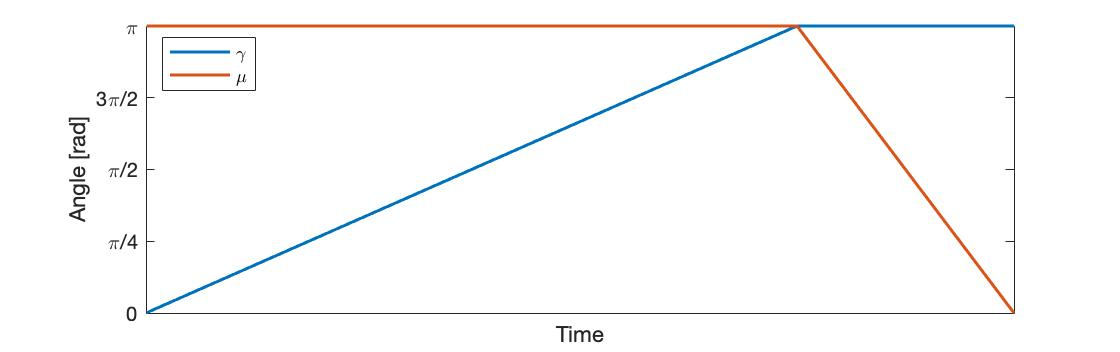
\includegraphics[width=\linewidth]{../matlab/paramEvolution.jpg}
\captionof{figure}{Angles evolution over time}
\label{fig:paramEvolution}
\vspace{0.5cm}

Note that for $\gamma$ the evolution is perfectly defined, as the increment of said angle needs to be positive in order to increase the flight altitude. Conversely, for $\mu$ the pilot could choose to rotate in the opposite direction thus changing $\mu$ from 0 to $-\pi$ instead - note that $\pi$ and $-\pi$ are equivalent -, and the result would be virtually the same.\\
Furthermore, in order to describe a perfect semicircle the angular speed $\dot{\gamma}$ needs to remain constant. This results in the necessary condition of gamma's evolution to be a straight slope. For $\mu$, however, the pilot could also perform the roll at non-constant rotating speed without this having an impact on the maneuver performance. This would be reflected as a curve on mu's temporal evolution, instead of a straight line.\\

All these
For the following computations, some values will be needed in order to numerically solve the Ordinal Differential Equation systems. The ENAERT T-35 Pillán, a Chilean military small aircraft and its data \cite{jane1969jane} have been taken as references.\\

\begin{center}
	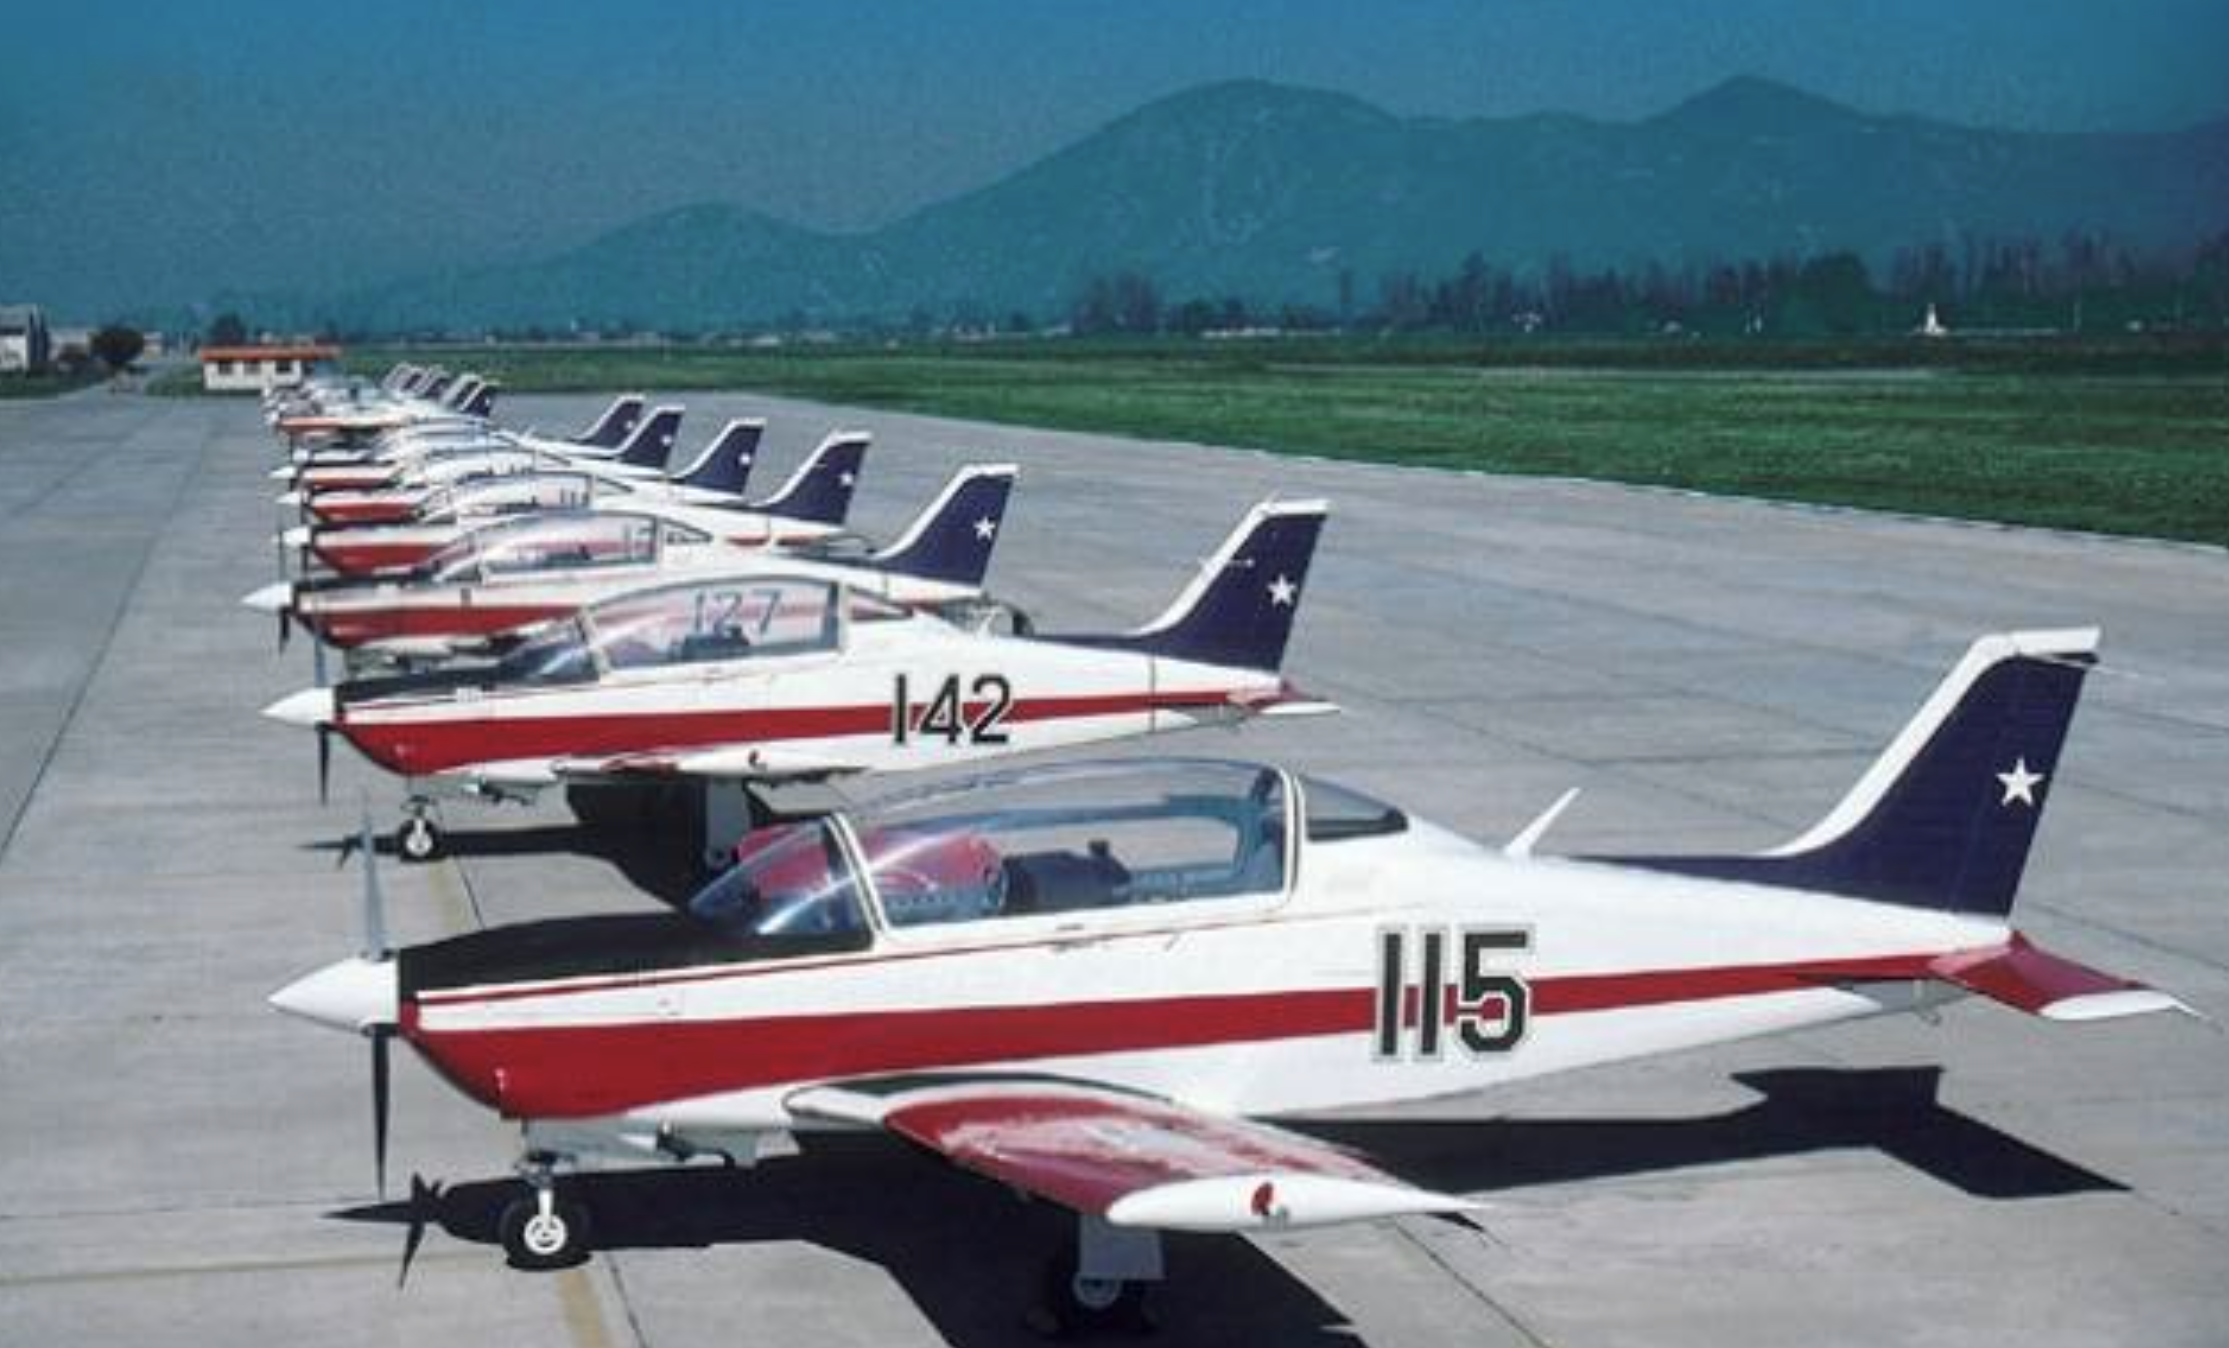
\includegraphics[width=0.9\linewidth]{figures/pillan}
	\vspace{0.5cm}
	\captionof{figure}{ENAERT T-35 Pillán. Extracted from \cite{defensa.com_2018}}\vspace{0.25cm}
\end{center}

The used information is:

\begin{center}
\begin{tabular}{|l|l||l|l|}\hline
	 & Value &   & Value\\ \hline \hline
	Mass & 1.300 kg& Wingspan & 8.84 m\\ \hline
	Airfoil & 63$_3$-414 & Wing area & 13.69 m$^2$ \\ \hline
	Stall s. & 31.94 m/s &  Cruise s. & 70.84 m/s\\ \hline
	Thrust &224 kW & Air den. & 1.225 kg/m$^3$ \\ \hline
	\multicolumn{4}{|c|}{$C_L=12\alpha+0.33$}\\ \hline	
\end{tabular}
\end{center}

The selected initial speed is of 70 m/s as the third phase of the maneuver requires a few less meters per second in order to be performed safely.

For the totality of the maneuver, the fixated parameters are the gas control lever ($\pi$) and the elevator ($\alpha$), which are set as constants at 1.5 kN and 0.3 rad respectively. From the remaining variables, the position coordinates evolution ($\Dot{x}$ and $\Dot{z}$) are always left as dependant in order to be solved by the ODE solver. With the obtained results, the trajectory is plot - see the following section Trajectory analysis, where both of them are studied in moer depth -.

\begin{equation} \label{eq:lift}
	L=\frac{1}{2}S\rho V(t)^2 C_L(\alpha)
\end{equation}
\begin{equation} \label{eq:drag}
	D=\frac{1}{2}S\rho V(t)^2 C_D(\alpha)
\end{equation}

\subsubsection*{Cruise flight}
\addcontentsline{toc}{subsection}{Cruise flight}
For the first and last phases, both cruise flight, the remaining variable (not counting $\Dot{x}$ and $\Dot{z}$) is velocity (V) alone.\\
As fixed thrust and elevator deflection are imposed, there are virtually no temporal changes affecting velocity. This results in constant speed or cruise flight, and a simple slope regarding the x-axis position. When computing both the lift and drag forces, these must be constant too - see equations \ref{eq:lift} and \ref{eq:drag} -.\\

Velocity being constant results in both lift and drag being constant too.
\begin{center}
	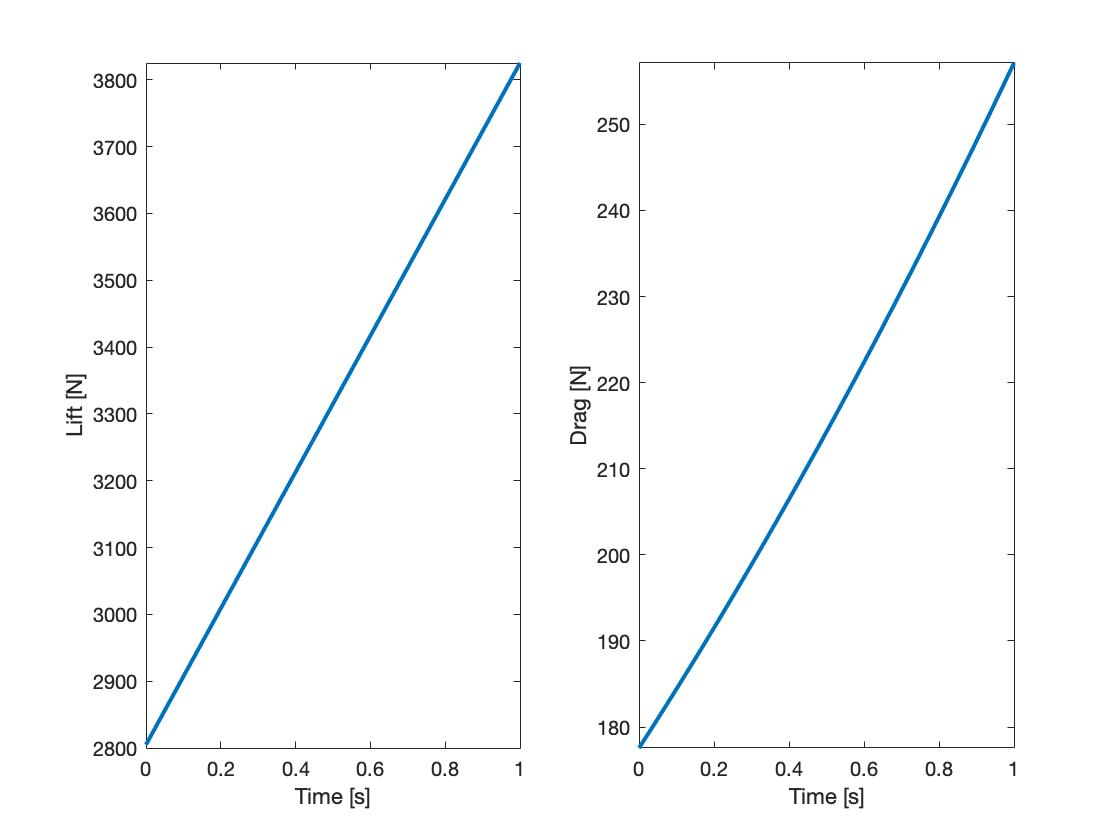
\includegraphics[width=\linewidth]{../matlab/1/liftdrag.jpg}
	\vspace{0.5cm}
	\captionof{figure}{Radius dependance on V and $\alpha$t. Own elaboration.}\vspace{0.25cm}
\end{center}

In regards of the general overview, cruise flight is quite straight forward, as both the speed and vertical position remain constant, and as velocity is linealry dependant on time, the displacement of the aricraft is linear as well.
\begin{center}
	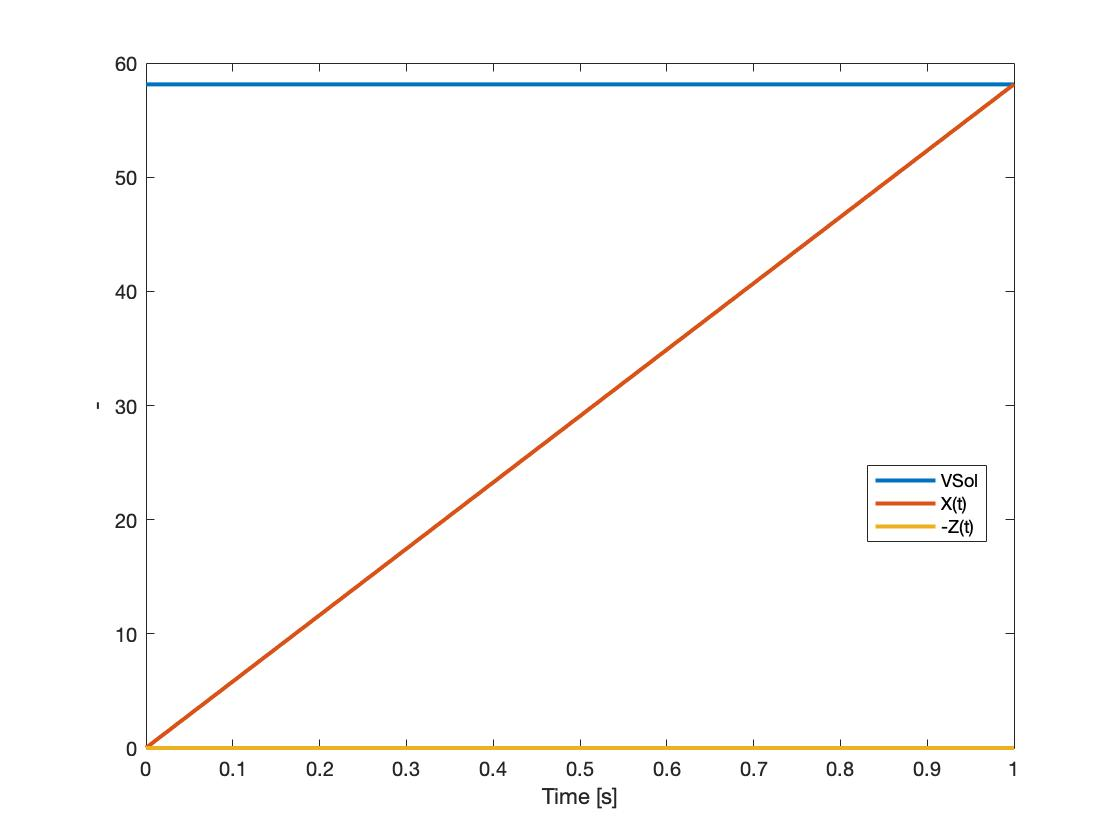
\includegraphics[width=\linewidth]{../matlab/1/1traj.jpg}
	\vspace{0.5cm}
	\captionof{figure}{Radius dependance on V and $\alpha$t. Own elaboration.}\vspace{0.25cm}
\end{center}

For the total time, the following integration from the first equation can be done:
\begin{align*}
	dt =& \frac{m}{T - D} dV\\
	\int dt= & \int \frac{m}{T - D} dV
	\intertext{Subsituting drag's definition from equation \ref{eq:drag} and operating for lineal aeordynamics,}
	= & \int_{V_0}^{V} \frac{m}{T - \frac{1}{2}\rho S V^2 (C_{D_0}+kC_L^2)} dV\\
	t_1=& \frac{m}{T - \frac{1}{2}\rho S V^2 (C_{D_0}+kC_L^2)} (V-V_0)
\end{align*}

\subsubsection*{Half loop}
\addcontentsline{toc}{subsection}{Half loop}
In order to work with the half loop part of the maneuver, some preliminary of the trajectory geometry is done.
The three force configurations during the maneuver correspond to the free body diagrams at stages 1, 2 and 3 (see Figure \ref{fig:immelmann-overview}). \vspace{0.5cm}

%\begin{minipage}{\textwidth}
	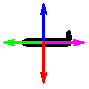
\includegraphics[width=0.3\linewidth]{figures/free-body-1.pdf} \hfill
%	\captionof{subfigure}{Angles evolution over time}
	\label{fig:free-body-1}
		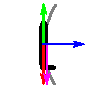
\includegraphics[width=0.3\linewidth]{figures/free-body-2.pdf}\hfill
%	\captionof{subfigure}{Angles evolution over time}
	\label{fig:free-body-2}
		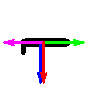
\includegraphics[width=0.3\linewidth]{figures/free-body-3.pdf}
%	\captionof{subfigure}{Angles evolution over time}
	\label{fig:free-body-3}
	\vspace{0.5cm}
	\captionof{figure}{Free body diagrams during the semiloop. Own elaboration.}\vspace{0.25cm}
		\label{fig:3avions}
%\end{minipage}

Note that at all times the lift behaves as the centripetal force, thus indicating that both the velocity and radius limitations to perform the Immelmann turn are inherent to the wing design and its maximum and minimum lift generation.\\
AS the motion will be circular, the normal and tangential accelerations will follow:
\begin{align*}
	a_n=&\frac{V^2}{R}=V\dot{\gamma}=\dot{\gamma}^2R&a_t=V^2R
\end{align*}
As a result, the radius can be writen as a function of the angle of attack. By operating with the third equation of system number \ref{eq:semicircle}, which is in wind system of reference, very convenient as is also polar set of axis:
\begin{align*}
	L=&m\left(\frac{V^2}{R}+g\cos(\gamma)\right)\\
	\frac{1}{2}\rho S V^2 C_L(\alpha)=&m\left(\frac{V^2}{R}+g\cos(\gamma)\right)\\
	R=&\frac{2mV^2}{2W\cos(\gamma)+\rho S V^2 C_L(\alpha)}
\end{align*}
As the plane must describe a semicircle, the radius must be constant.

\begin{center}
	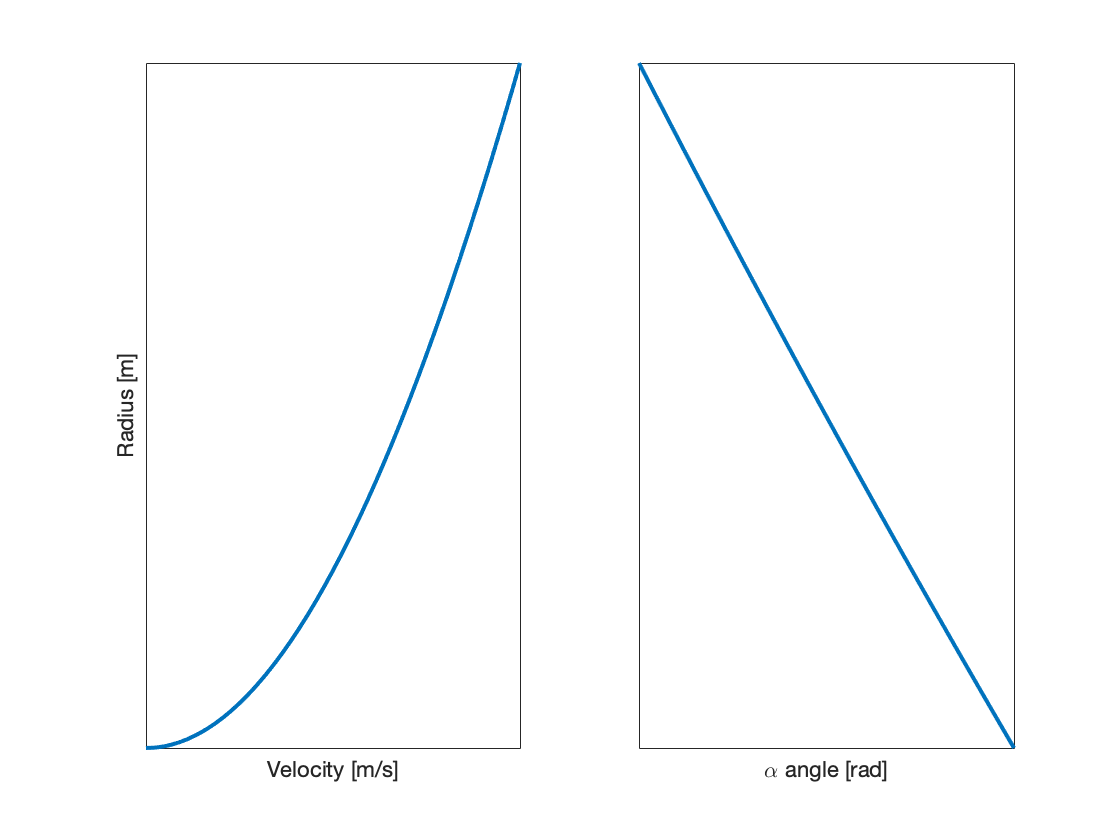
\includegraphics[width=\linewidth]{../matlab/radius.png}
	\vspace{0.5cm}
	\captionof{figure}{Radius dependance on V and $\alpha$t. Own elaboration.}\vspace{0.25cm}
\end{center}

For this phase the evolution of $\gamma$ will be imposed. By using the following conditions:
\begin{itemize}
	\item Must begin at 0 and end at $\pi$ rad
	\item Must have a linear evolution troughout time - in order not to overcomplicate the problem -
	\item Must be compatible with circular accelerations, as the ideal performance of the maneuver would require the half loop to be a semicirle
\end{itemize}

From these it can clearly be deucted that the basic model for a slope will be required
\[\gamma(t)=At+B\]
And the rest of conditions define the parameters A and B such that the resulting expression is obtained:
\begin{align}
	\gamma(t)=&\frac{V_0}{R}t & &or& \gamma(t)=&\frac{V_0}{R}t + \pi-\frac{V_0}{R}tf 
\end{align}
Where the finishing time of \textit{tf} would be $tf=\pi/V_0$.\\
Note that $V_0$ instead of V(t) has been employed. This is in order to ensure the linearity, although a time dependant velocity could be used too. This would lead to a concatenation of curves for the loop, and not a semicirle.\\

Given that the determined parameters are therefore the gas control lever ($\pi$) and the elevator ($\alpha$), with the same values as for the previous phase - 1.5 kN and 0.3 rad respectively -, but also $\gamma$ is, the only variable to study is the velocity. Nothe that the position coordinates evolution ($\Dot{x}$ and $\Dot{z}$) are explored in the following section: Trajectory analysis.\\

For this phase, the velocity must follow a non-linear evolution as it is dependant on both trigonometric and squared terms in the equations, see $\gamma$ and the lift and drag forces definitions in equations \ref{eq:lift} and \ref{eq:drag}. \\
As the previous shcemes in Figure \ref{fig:3avions} show, at the vertical flight after a quarter of loop, the velocity slows its rate of increase at that point. This inflection point is the consequence of the weight force switching the aircraft's axis for $\gamma=\pi/2$ thus forcing a force redistribution in order to mantain equilibrium.\\
As Figure \ref{fig:radivelo} shows, it is worth noting too that the higher the initial speed solely modifies the placement of the curve in the plot, but has no effect on its characteristics. Althoug it is not clearly shown in the plot, the time is reduced too. On the contrary, for a fixed velocity, different radii have a more noticeable impact on the performance of the semiloop. As greater radius require more time to get to the quarter loop point - for the same initial speed -, the local velocity maximum prior to the $\gamma=\pi/2$ state is higher the greater the radius. Although both the local maximum and the finoshing speed are higher, the greater the radius the longer it takes to complete the half loop.

\begin{center}
	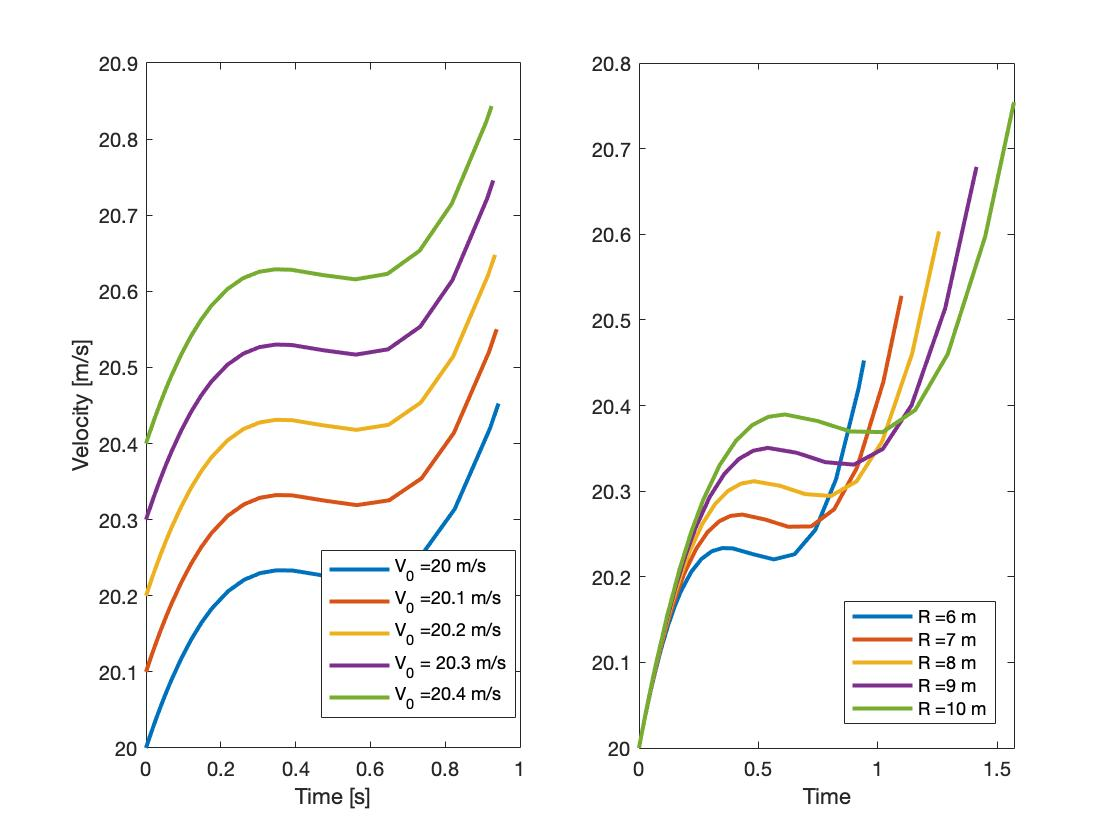
\includegraphics[width=\linewidth]{../matlab/radivelo.jpg}
	\vspace{0.5cm}
	\captionof{figure}{Radii and velocity dependencies on the half loop. Own elaboration.}\vspace{0.25cm}
	\label{fig:radivelo}
\end{center}

Both the lift and drag are affected by this velocity oscillation, but its mangnitude is rather small when compared to the rest of the parameters'.

\begin{center}
	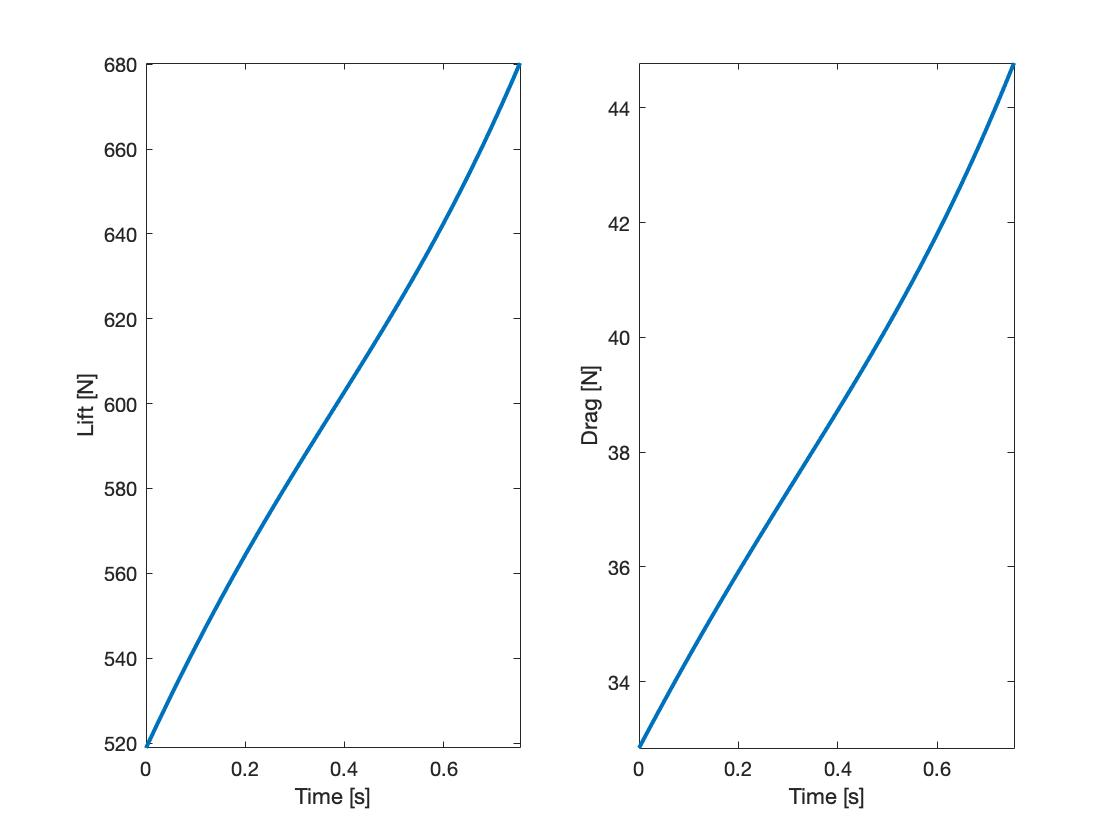
\includegraphics[width=\linewidth]{../matlab/2/liftdrag.jpg}
	\vspace{0.5cm}
	\captionof{figure}{Lift and drag on the half loop. Own elaboration.}\vspace{0.25cm}
	\label{fig:Ld2}
\end{center}

Lastly, both of the position coordinates evolution ($\Dot{x}$ and $\Dot{z}$) evolve as expected, this is, highly dependant on $\gamma$. As this angle ranges from 0 to $\pi$, both coordinates follow reasonable behaviours. It is also clearly shown that the speed remains fairly constant during this part of the maneuver too.

\begin{center}
	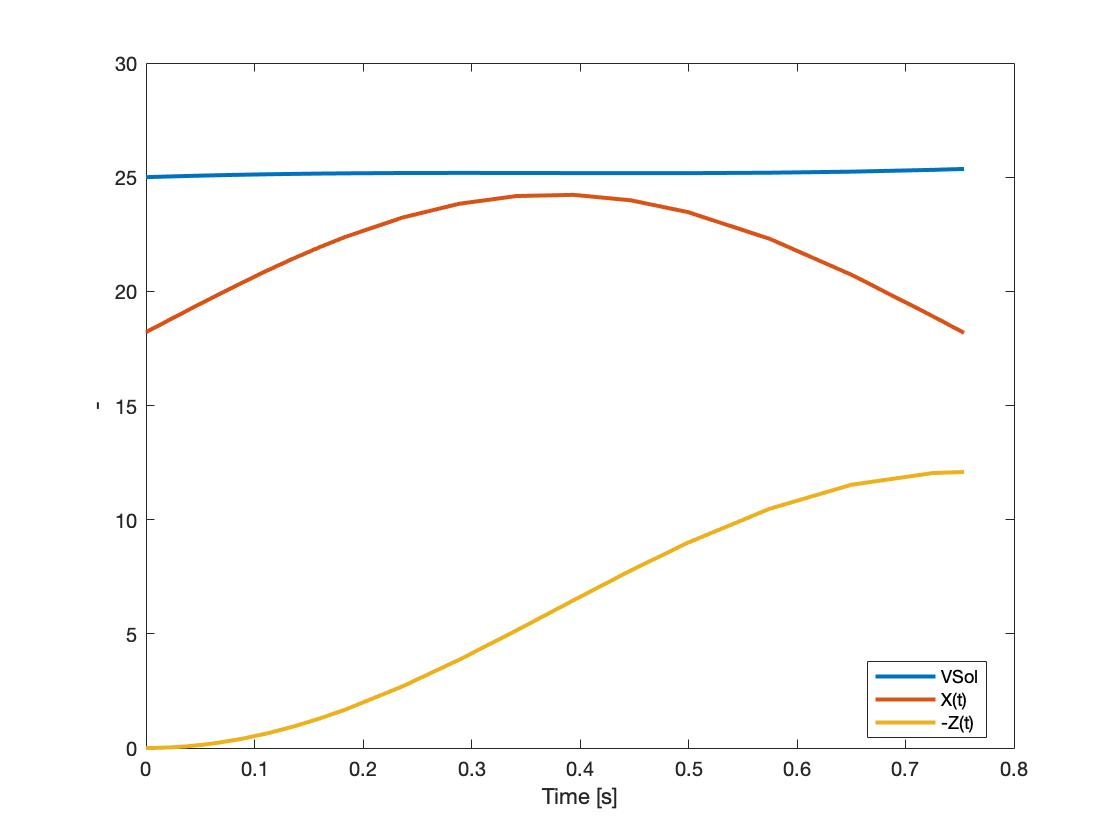
\includegraphics[width=\linewidth]{../matlab/2/trajectory.jpg}
	\vspace{0.5cm}
	\captionof{figure}{Radii and velocity dependencies on the half loop. Own elaboration.}\vspace{0.25cm}
	\label{fig:2traj}
\end{center}
For time integration in this case 
\begin{align*}
	\begin{cases}
		\frac{\partial V}{\partial t}=&\frac{1}{m}\left(T - D -mg\sin\gamma\right)\\
		\frac{\partial \gamma}{\partial t}=&\frac{1}{mV}\left(L-mg\cos\gamma\right)
	\end{cases}
\end{align*}
As during this phase the angle $\gamma$ must evolve from 0 to $\pi$ rad -for simplification purposes we will work with a linear model - and, as previously stated, the circular motion accelerations have been assumed to apply, we can write:
\begin{align*}
	\gamma(t) =& \frac{V}{R}t & \frac{\partial \gamma(t)}{\partial t}=\frac{V}{R}
\end{align*}
\begin{align*}
	dt =& \frac{m}{T - D -mg\sin\gamma} dV\\
	\int dt= & \int \frac{m}{T - D -mg\sin\gamma} dV
	\intertext{Subsituting drag's definition from equation \ref{eq:drag} and operating for lineal aeordynamics,}
	= & \int \frac{m}{T - \frac{1}{2}\rho S V^2 (C_{D_0}+kC_L^2) -mg\sin\gamma} dV
	\intertext{Substituting ,}
\end{align*}
%%%%%%%%%%%%%%%%%%%%%%%%%%%%%%%%%%%%%%%%%%%%%%
\subsubsection*{Roll}
\addcontentsline{toc}{subsection}{Roll}
Similarly to the half loop, for this phase a part of the known fixed parameters; gas control lever ($\pi$) and elevator deflection ($\alpha$) more conditioning is needed. In this case, the angle is the roll angle; $\mu$. As previouslt done for $\gamma$, the conditions for $\mu$ are:

\begin{itemize}
	\item Must begin at $\pi$ (or -$\pi$) and end at 0 rad
	\item Must have a linear evolution troughout time - in order not to overcomplicate the problem -
\end{itemize}

From these it can clearly be deucted that the basic model for a slope will be required
\[\mu(t)=At+B\]
As we are missing some conditions to deremine the rate at which the aircraft should roll, the selection is based on the aircraft's structural capacities. For aerobatic aricrafts the rolls must be performed at approximately 120 knots for full aileron rolls and a rotating velocity of 7 m/s at the tip of the wing. With this data and the wingspan we can extract the expressions:
\begin{align}
	\mu(t)=&-\frac{V_{tip}}{b/2}t+\pi \\
	\intertext{or} 
	\mu(t)=&-\frac{V_{tip}}{b/2}t+\pi-\frac{V_{tip}}{b/2}tf
\end{align}
Where the finishing time of \textit{tf} would be $tf=\pi \frac{b/2}{V_{tip}}$.\\
If the evolution of $\mu$ is considered, though, it can be seen that between $\pi$ and $\pi/2$ its trigonometric value for cosinus is negative. For the equation that yields the velocity - \textit{squared} velocity - this is rather problematic.\\

\begin{center}
	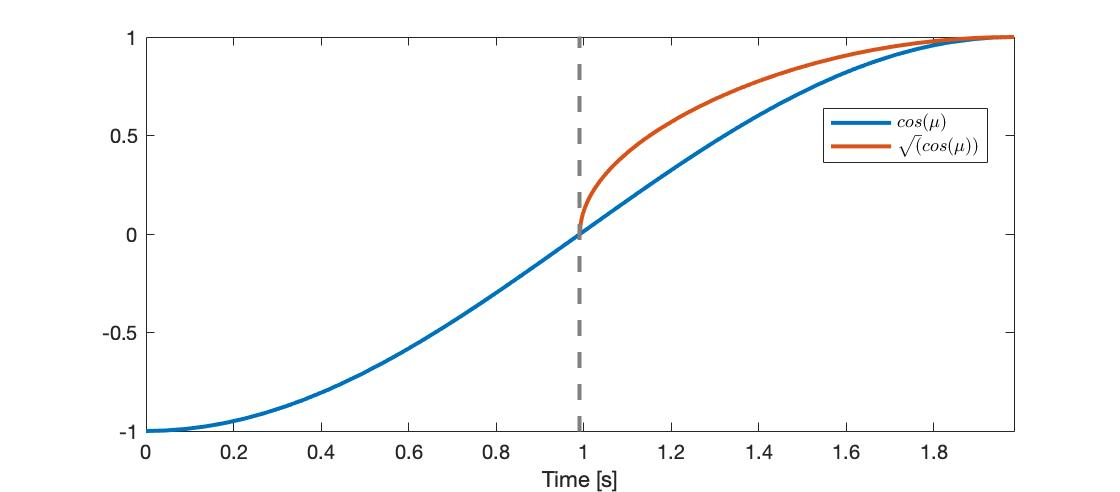
\includegraphics[width=\linewidth]{../matlab/3/sqrt.jpg}
	\vspace{0.5cm}
	\captionof{figure}{Unsolvable domain of part of the trajectory. Own elaboration.}\vspace{0.25cm}
\end{center}

For this reason, the computations have been done only for half of the phase, understanding that the remaining quarter of roll is symmetric.

The velocity is deeply conditioned by the values that $\mu$ acquires throughout the roll, even tending to infinity due to the previously mentioned trigonometric properties. In reality, we can assume a small variation of the total lift and drag, whoch would be oscillating between the lower values of the plots from Figure \ref{fig:ld3}.
\begin{center}
	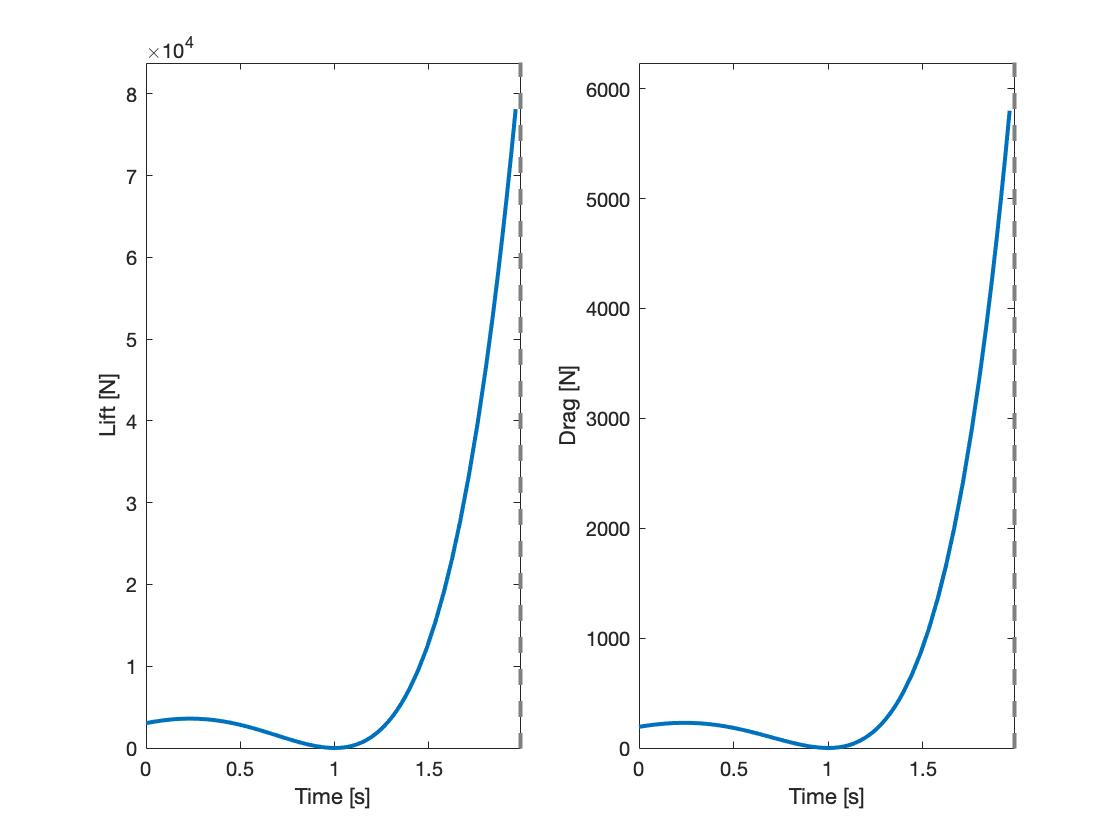
\includegraphics[width=\linewidth]{../matlab/3/liftdrag.jpg}
	\vspace{0.5cm}
	\captionof{figure}{Unsolvable domain of part of the trajectory. Own elaboration.}\vspace{0.25cm}
	\label{fig:ld3}
\end{center}

For the general overview:
\begin{center}
	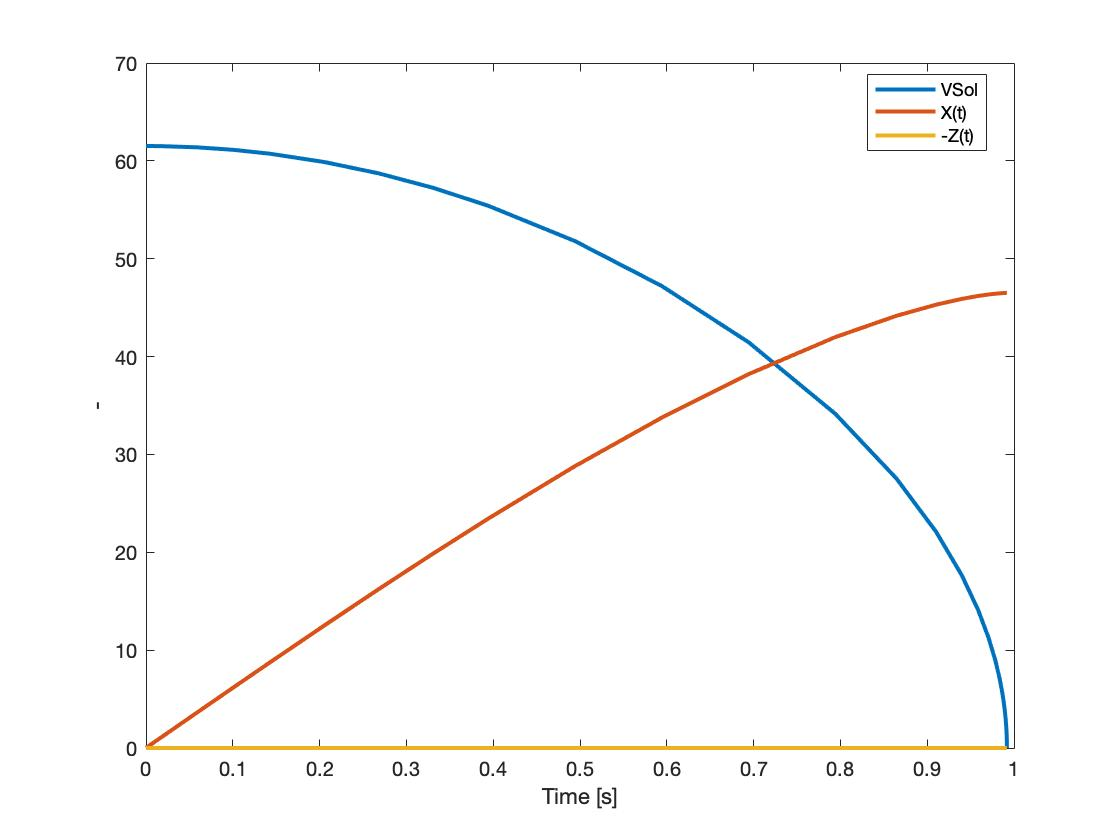
\includegraphics[width=\linewidth]{../matlab/3/3traj.jpg}
	\vspace{0.5cm}
	\captionof{figure}{Radii and velocity dependencies on the half loop. Own elaboration.}\vspace{0.25cm}
	\label{fig:3traj}
\end{center}

The total velocity and x(t) would continue simetrically; the velocity would rapidly increase again and the position would exit the inflection point to keep increasing again.\\

Temporal integration is exactly equal to the cruise phase one, as the roll does not have an effect on the temporal derivatives.
\begin{align*}
	dt =& \frac{m}{T - D} dV\\
	\int dt= & \int \frac{m}{T - D} dV
	\intertext{Subsituting drag's definition from equation \ref{eq:drag} and operating for lineal aeordynamics,}
	= & \int_{V_0}^{V} \frac{m}{T - \frac{1}{2}\rho S V^2 (C_{D_0}+kC_L^2)} dV\\
	t_1=& \frac{m}{T - \frac{1}{2}\rho S V^2 (C_{D_0}+kC_L^2)} (V-V_0)
\end{align*}

Note that this phase of the maneuver is perhaps the most idealised, as a roll is an unbalanced maneuver. Because of the aircraft stability design adverse yaw appears from the very beginning. In a nutshell,  an aircraft performing an aileron roll will actually fly along a slightly helical path, and a very light, positive g force will be maintained.

\subsection*{Trajectory analysis} 
\addcontentsline{toc}{section}{Trajectory analysis}
The expected result of the trajectory is portrayed in the following image:

\begin{center}
	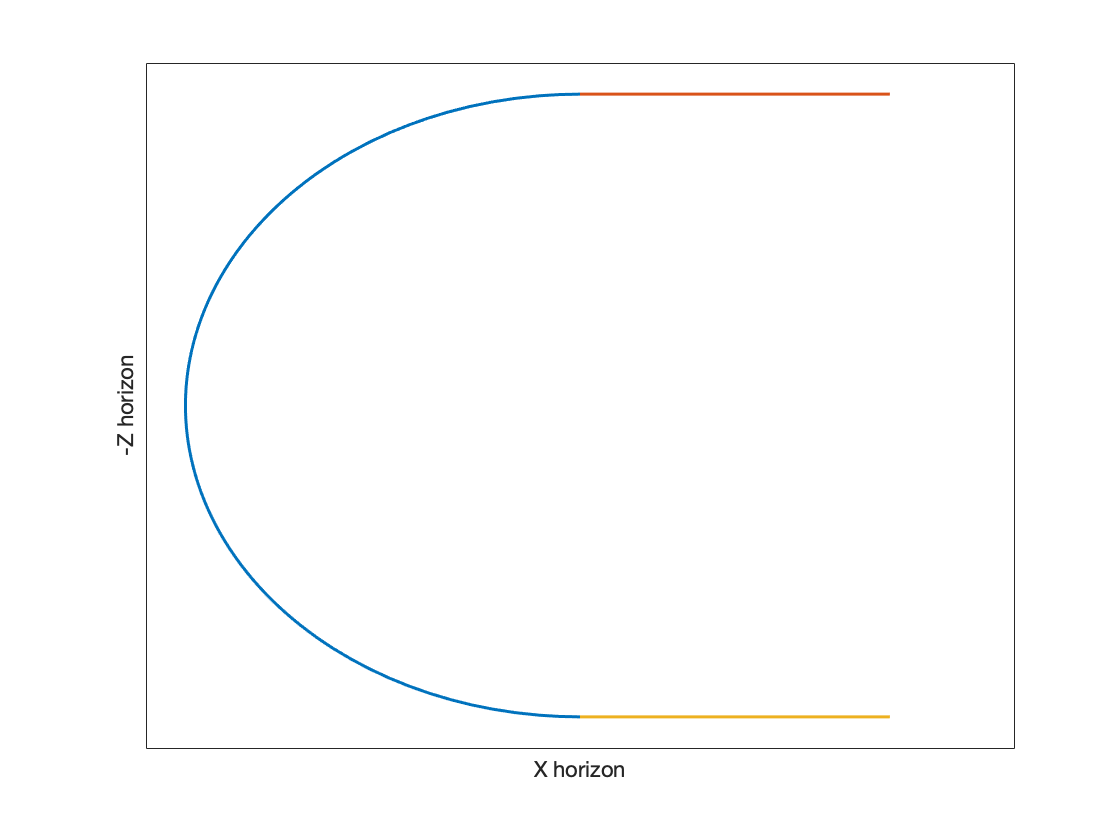
\includegraphics[width=\linewidth]{../matlab/trajectory.png}
	\vspace{0.5cm}
	\captionof{figure}{Expected trajectory output. Own elaboration.}\vspace{0.25cm}
\end{center}

We can consider the maneuver coordinates:
\begin{align*}
	\dot{x}_e=&V\cos\gamma&&&	x_e=&Vt\cos\gamma \\
	\dot{y}_e=&0& \rightarrow&&	y_e=&0\\
	\dot{x}_e=&-V\sin\gamma&&&z_e=&-Vt\sin\gamma
\end{align*}

From the computational results obtained from ODE solvers, the following plots represent the trajectory:
\begin{center}
	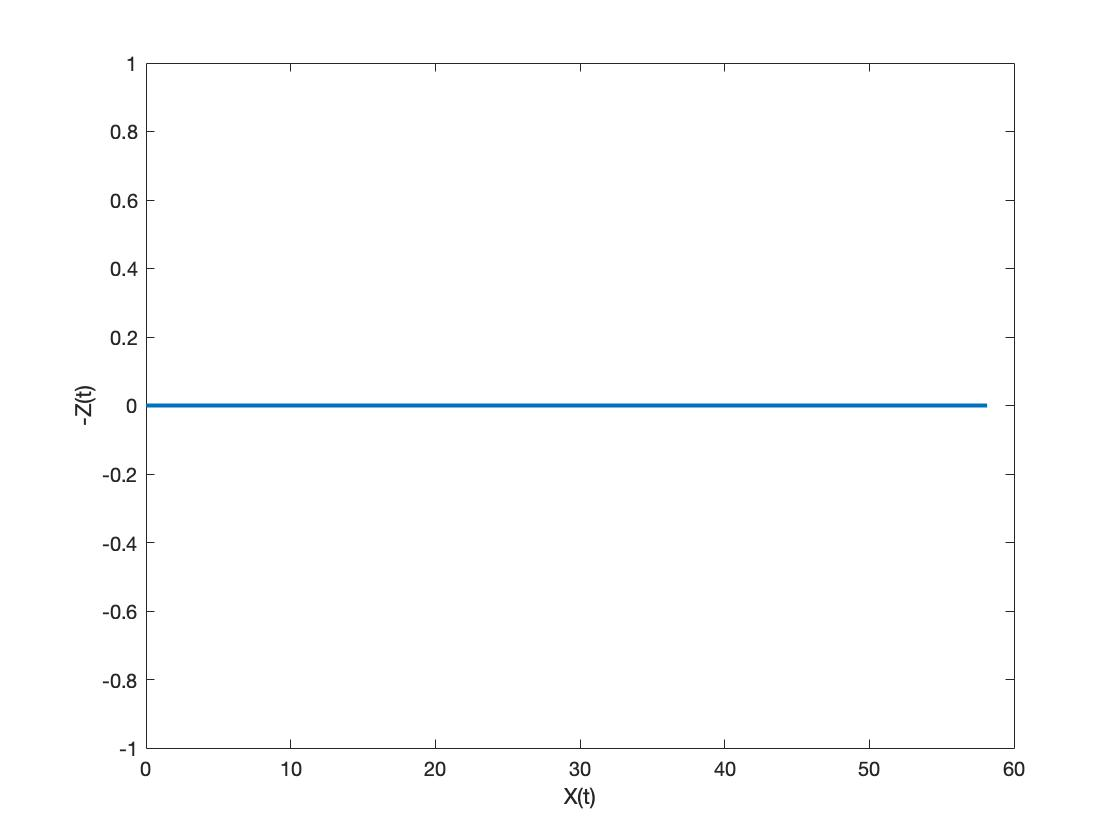
\includegraphics[width=\linewidth]{../matlab/t1.jpg}
	\vspace{0.25cm}
	\captionof{figure}{Trajectory output for cruise flight. Own elaboration.}\vspace{0.25cm}
\end{center}

\begin{center}
	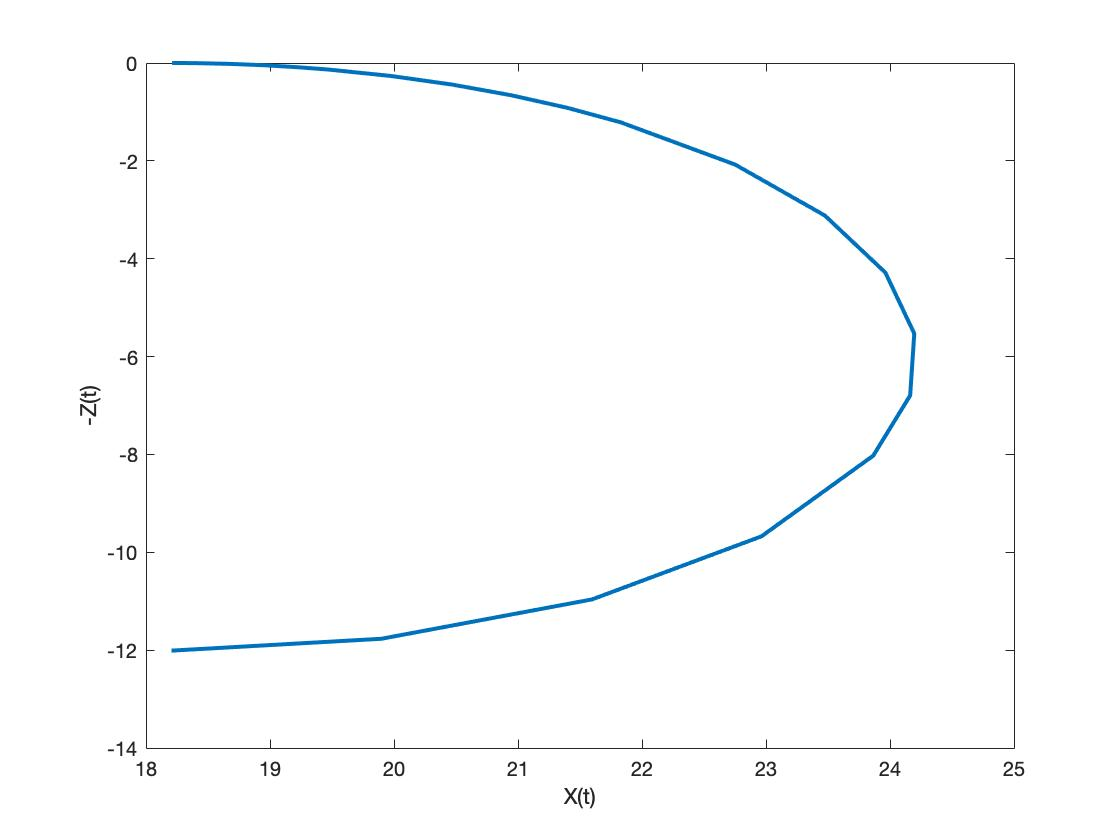
\includegraphics[width=\linewidth]{../matlab/t2.jpg}
	\vspace{0.25cm}
	\captionof{figure}{Trajectory output for the semiloop. Own elaboration.}\vspace{0.25cm}
\end{center}

\begin{center}
	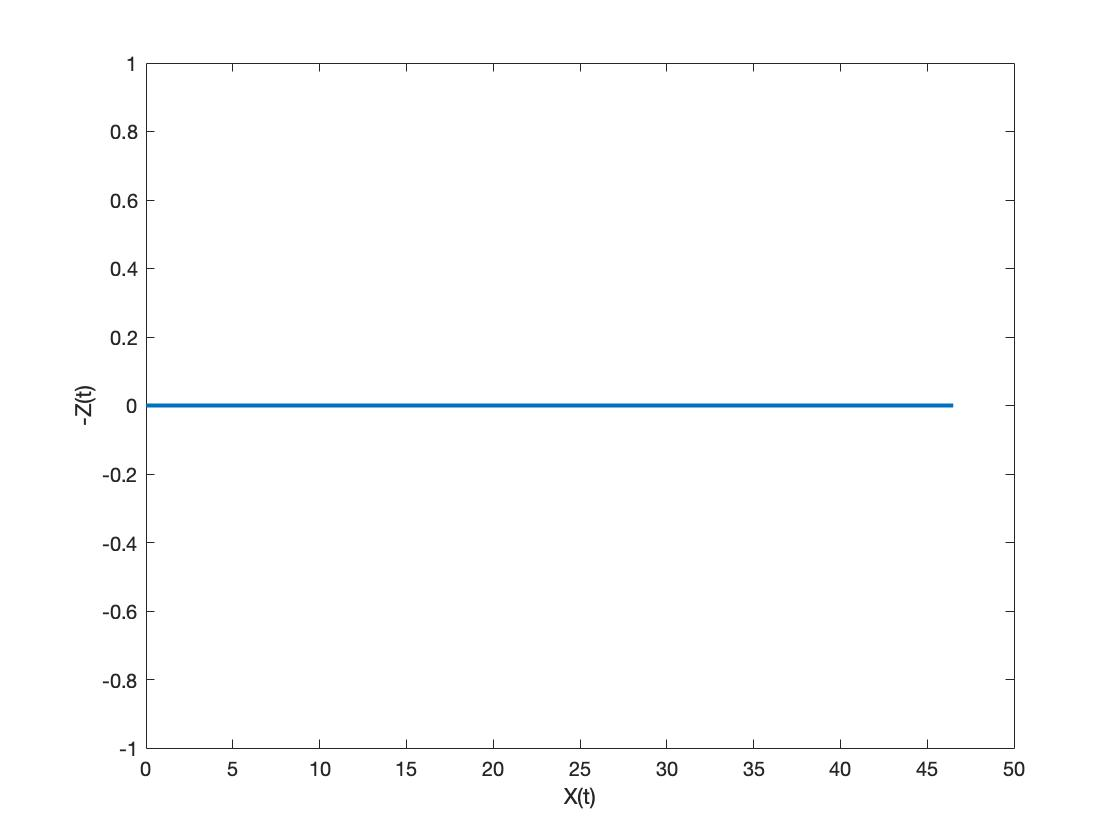
\includegraphics[width=\linewidth]{../matlab/t3.jpg}
	\vspace{0.25cm}
	\captionof{figure}{Trajectory output for the roll. Own elaboration.}\vspace{0.25cm}
\end{center}

The obtained results fit perfectly with the expected outuput.